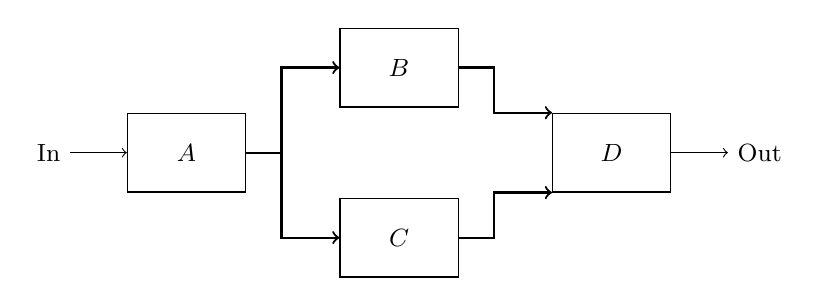
\begin{tikzpicture}[scale=0.9, every node/.style={font=\small}]
  % Boxes
  \node[draw, rectangle, minimum width=1.5cm, minimum height=1cm] (A) at (0,0) {$A$};
  \node[draw, rectangle, minimum width=1.5cm, minimum height=1cm] (B) at (3,1.2) {$B$};
  \node[draw, rectangle, minimum width=1.5cm, minimum height=1cm] (C) at (3,-1.2) {$C$};
  \node[draw, rectangle, minimum width=1.5cm, minimum height=1cm] (D) at (6,0) {$D$};

  % Wires
  \draw[->, thick] (A.east) -- ++(0.5,0) |- (B.west);
  \draw[->, thick] (A.east) -- ++(0.5,0) |- (C.west);
  \draw[->, thick] (B.east) -- ++(0.5,0) |- (D.north west);
  \draw[->, thick] (C.east) -- ++(0.5,0) |- (D.south west);

  % Inputs/Outputs
  \draw[<-] (A.west) -- ++(-0.8,0) node[left] {In};
  \draw[->] (D.east) -- ++(0.8,0) node[right] {Out};
\end{tikzpicture}